\documentclass[10pt,a4paper]{article}
\usepackage{tocloft}
\usepackage{commons/course}
\usepackage{booktabs}
\usepackage{graphicx}
\usepackage{tikz}
\usetikzlibrary{arrows.meta,positioning,calc}

\definecolor{keywordstyle}{rgb}{0.0, 0.4, 0.8}
\definecolor{stringstyle}{rgb}{0.9, 0.17, 0.31}
\definecolor{commentstyle}{rgb}{0.1, 0.6, 0.2}
\definecolor{numberstyle}{rgb}{0.4, 0.4, 0.4}
\definecolor{backgroundcolor}{rgb}{0.94, 0.97, 1.0}

\lstdefinelanguage{ShellLike}{
	morekeywords={PASS,FAIL,Passed,Failed,Running,Loading,summary,iverilog},
	sensitive=false,
	morecomment=[l]{\#},
	morestring=[b]",
}

\lstset{
	language=ShellLike,
	basicstyle=\ttfamily\scriptsize,
	keywordstyle=\color{keywordstyle}\bfseries,
	stringstyle=\color{stringstyle},
	commentstyle=\color{commentstyle},
	numbers=none,
	keepspaces=true,
	tabsize=2,
	showspaces=false,
	showstringspaces=false,
	showtabs=false,
	breaklines=true,
	breakatwhitespace=false,
	frame=single,
	backgroundcolor=\color{backgroundcolor},
}

\lstdefinestyle{verilog}{
	language=Verilog,
	basicstyle=\ttfamily\scriptsize,
	keywordstyle=\color{keywordstyle}\bfseries,
	commentstyle=\color{commentstyle},
	stringstyle=\color{stringstyle},
	numbers=left,
	numberstyle=\tiny\color{numberstyle},
	frame=single,
	backgroundcolor=\color{backgroundcolor},
	breaklines=true,
	tabsize=2,
}

\newlistof{listofproblems}{lop}{\normalsize فهرست مسائل}
\newcommand{\addproblem}[1]{\addcontentsline{lop}{listofproblems}{\protect\numberline{}#1}}

\begin{document}

\سربرگ{آزمایش سوم}{توصیف جریان داده (مقایسه‌کننده‌ی آبشاری و سریال)}{}{استاد: دکتر انصاری}

\subsubsection*{خلاصه}

در این آزمایش دو مدار مقایسه‌کننده با توصیف \textbf{جریان داده} (\lr{assign}) در \lr{Verilog} پیاده‌سازی شده‌اند و با \lr{Icarus Verilog} (\lr{iverilog}/\lr{vvp}) صحت‌سنجی شده‌اند:

\begin{enumerate}
  \item یک \lr{Cascadable 1-bit comparator} کاملا ترکیبی با \lr{assign}، و سپس یک مقایسه‌کننده‌ی چهاربیتی سلسله‌مراتبی ساخته‌شده از چهار نمونه‌ی آن (\lr{MSB}$\to$\lr{LSB}).
  \item یک مقایسه‌کننده‌ی \textbf{سریال} ترتیبی که بیت‌به‌بیت (از پرارزش‌ترین بیت) دو عدد را می‌گیرد و در هر پالس ساعت نتیجه‌ی مقایسه‌ی تا همین‌جا را روی خروجی‌های \lr{GT}/\lr{EQ}/\lr{LT} می‌گذارد. برای این قسمت دو نسخه نوشته شده: نسخه‌ی \textbf{A} (منطق next-state با \lr{assign} + فلیپ‌فلاپ لبه‌حساس با \lr{always}) و نسخه‌ی \textbf{B} (تمام ماژول فقط با \lr{assign}، با زوج \lr{latch} مسترـ‌اسلیو برای نگهداری حالت).
\end{enumerate}

\subsubsection*{هدف آزمایش}

\begin{itemize}
  \item تمرین توصیف جریان داده با دستور \lr{assign} برای مدار ترکیبی.
  \item طراحی سلسله‌مراتبی: بلوک ۱بیتی قابل آبشار، سپس ساخت ۴بیتی از آن.
  \item توصیف مدار ترتیبی با منطق next-state به سبک جریان داده، و مقایسه‌ی دو روش نگهداری حالت (فلیپ‌فلاپ لبه‌حساس در برابر زوج \lr{latch} فقط با \lr{assign}).
  \item صحت‌سنجی با \lr{testbench} و شبیه‌ساز \lr{iverilog}.
\end{itemize}

\pagebreak
\subsubsection*{قسمت ۱: مقایسه‌کننده‌ی ۱بیتی آبشاری}

\begin{center}
\begin{tabular}{@{}lll p{7.5cm}@{}}
\toprule
\textbf{سیگنال} & \textbf{جهت} & \textbf{پهنا} & \textbf{توضیح} \\
\midrule
A, B & ورودی & ۱ & بیت‌های همین طبقه \\
GT\_in, EQ\_in, LT\_in & ورودی & ۱ & نتیجه‌ی cascade از بیت‌های پرارزش‌تر \\
GT\_out, EQ\_out, LT\_out & خروجی & ۱ & نتیجه‌ی به‌روز تا این بیت \\
\bottomrule
\end{tabular}
\end{center}

دانهٔ اول (قبل از \lr{MSB}) با $(GT,EQ,LT)=(0,1,0)$ تغذیه می‌شود؛ یعنی تا الان برابر. معادلات جریان داده:

\[
\begin{aligned}
EQ_{out} &= EQ_{in} \land \lnot(A \oplus B)\\
GT_{out} &= GT_{in} \lor (EQ_{in} \land A \land \lnot B)\\
LT_{out} &= LT_{in} \lor (EQ_{in} \land \lnot A \land B)
\end{aligned}
\]

یعنی فقط وقتی هنوز برابر بوده‌ایم اجازه‌ی تصمیم جدید داریم؛ بعد از تصمیم \lr{GT} یا \lr{LT}، همان مقدار از طبقه‌های بعدی عبور می‌کند.

\begin{latin}
\begin{lstlisting}[style=verilog]
assign EQ_out = EQ_in & ~(A ^ B);
assign GT_out = GT_in | (EQ_in & A & ~B);
assign LT_out = LT_in | (EQ_in & ~A & B);
\end{lstlisting}
\end{latin}

\subsubsection*{قسمت ۱: مقایسه‌کننده‌ی ۴بیتی سلسله‌مراتبی}

چهار نمونه‌ی \lr{cascadable\_1bit\_comparator} به زنجیره وصل شده‌اند:

\begin{center}
\begin{latin}
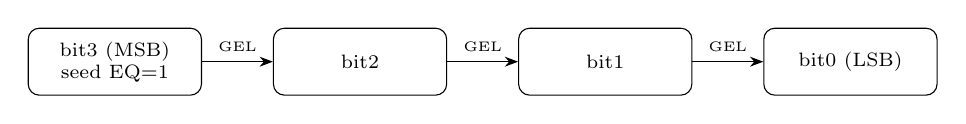
\begin{tikzpicture}[
  box/.style={draw, rounded corners, minimum width=2.2cm, minimum height=0.85cm, align=center, font=\scriptsize},
  >=Stealth, node distance=0.55cm and 0.9cm
]
  \node[box] (u3) {bit3 (MSB)\\seed EQ=1};
  \node[box, right=of u3] (u2) {bit2};
  \node[box, right=of u2] (u1) {bit1};
  \node[box, right=of u1] (u0) {bit0 (LSB)};
  \draw[->] (u3) -- (u2) node[midway,above,font=\tiny]{GEL};
  \draw[->] (u2) -- (u1) node[midway,above,font=\tiny]{GEL};
  \draw[->] (u1) -- (u0) node[midway,above,font=\tiny]{GEL};
\end{tikzpicture}
\end{latin}
\end{center}

مدار کاملا ترکیبی است (بدون کلاک). خروجی نهایی از طبقه‌ی \lr{LSB} برداشته می‌شود.

\subsubsection*{قسمت ۲: مقایسه‌کننده‌ی سریال}

\begin{center}
\begin{tabular}{@{}lll p{7.8cm}@{}}
\toprule
\textbf{سیگنال} & \textbf{جهت} & \textbf{پهنا} & \textbf{توضیح} \\
\midrule
clk & ورودی & ۱ & کلاک \\
reset & ورودی & ۱ & ریست ناهم‌گام فعال‌بالا \\
A, B & ورودی & ۱ & بیت جاری (ترتیب \lr{MSB}-اول) \\
GT, EQ, LT & خروجی & ۱ & نتیجه‌ی مقایسه تا بیت‌های دیده‌شده \\
\bottomrule
\end{tabular}
\end{center}

وضعیت با دو بیت $(eq_q, gt_q)$ کد می‌شود: بعد از ریست $(1,0)$ یعنی \lr{EQ}؛ $(0,1)$ یعنی \lr{GT}؛ $(0,0)$ یعنی \lr{LT}. معادلات next-state (برای هر دو نسخه یکسان):

\[
\begin{aligned}
eq_d &= eq_q \land \lnot(A \oplus B)\\
gt_d &= gt_q \lor (eq_q \land A \land \lnot B)\\
LT &= \lnot eq_q \land \lnot gt_q
\end{aligned}
\]

\paragraph{نسخه‌ی A --- \lr{serial\_comparator\_ff}.}
منطق بالا با \lr{assign}، و دو فلیپ‌فلاپ با \lr{always @(posedge clk or posedge reset)}. خروجی‌ها روی لبه‌ی بالارونده به‌روز می‌شوند.

\paragraph{نسخه‌ی B --- \lr{serial\_comparator\_assign}.}
طبق متن آزمایش، کل ماژول فقط \lr{assign} است (بدون \lr{always} و بدون نمونه‌سازی زیرماژول). نگهداری حالت با زوج \lr{latch} مسترـ‌اسلیو:

\begin{itemize}
  \item وقتی \lr{clk=1}: مستر next-state را نمونه‌برداری می‌کند.
  \item وقتی \lr{clk=0}: اسلیو از مستر به‌روز می‌شود (خروجی‌ها اینجا عوض می‌شوند).
\end{itemize}

این رفتار معادل یک فلیپ‌فلاپ حساس به لبه‌ی پایین‌رونده است؛ در تست‌بنچ بیت‌ها هنگام \lr{clk=0} آماده می‌شوند، سپس یک سیکل کامل \lr{0$\to$1$\to$0} زده می‌شود و خروجی بعد از افت کلاک خوانده می‌شود -- همان قرارداد یک بیت در هر پالس برای هر دو نسخه.

\subsubsection*{شکل موج (هر دو نسخه، یک محرک)}

هر دو شکل‌موج از یک تست‌بنچ مشترک (\lr{tb\_serial\_wave}) با همان دنباله گرفته شده‌اند:
ابتدا $A{=}0100$ در برابر $B{=}0011$ (تصمیم \lr{GT} روی بیت دوم و چسبندگی آن)، سپس ریست وسط‌راه، سپس $A{=}0001$ در برابر $B{=}0010$ (تصمیم \lr{LT} و چسبندگی). تفاوت ظاهری فقط در لبهٔ به‌روزرسانی خروجی است: نسخهٔ A روی لبه‌ی بالارونده، نسخهٔ B روی لبه‌ی پایین‌رونده.

\begin{center}
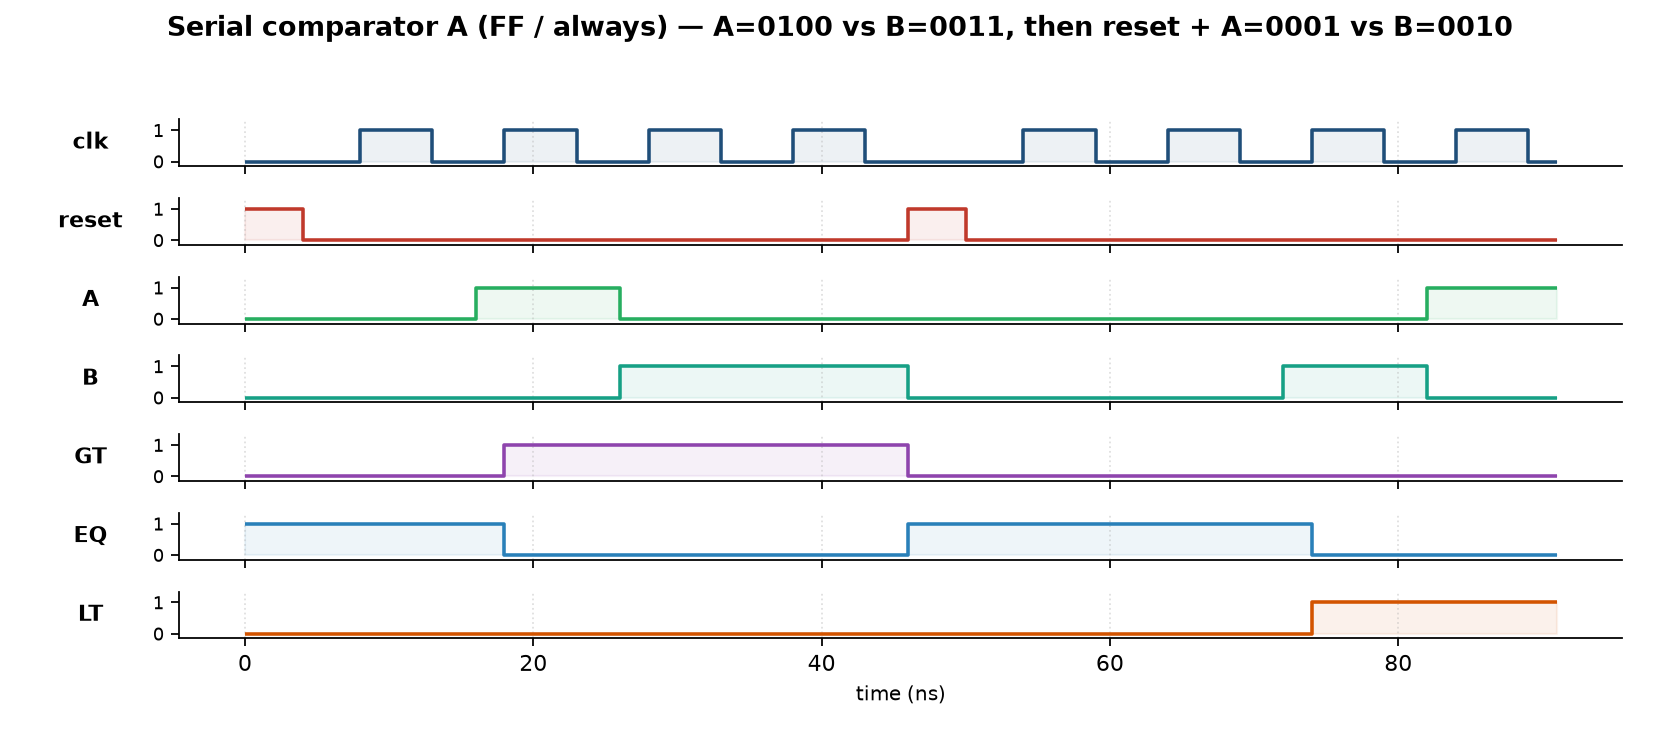
\includegraphics[width=\textwidth]{figs/wave_serial_ff.png}\\[0.4em]
{\small شکل ۱ --- نسخهٔ A (\lr{serial\_comparator\_ff}): فلیپ‌فلاپ با \lr{always @(posedge clk)}}
\end{center}

\begin{center}
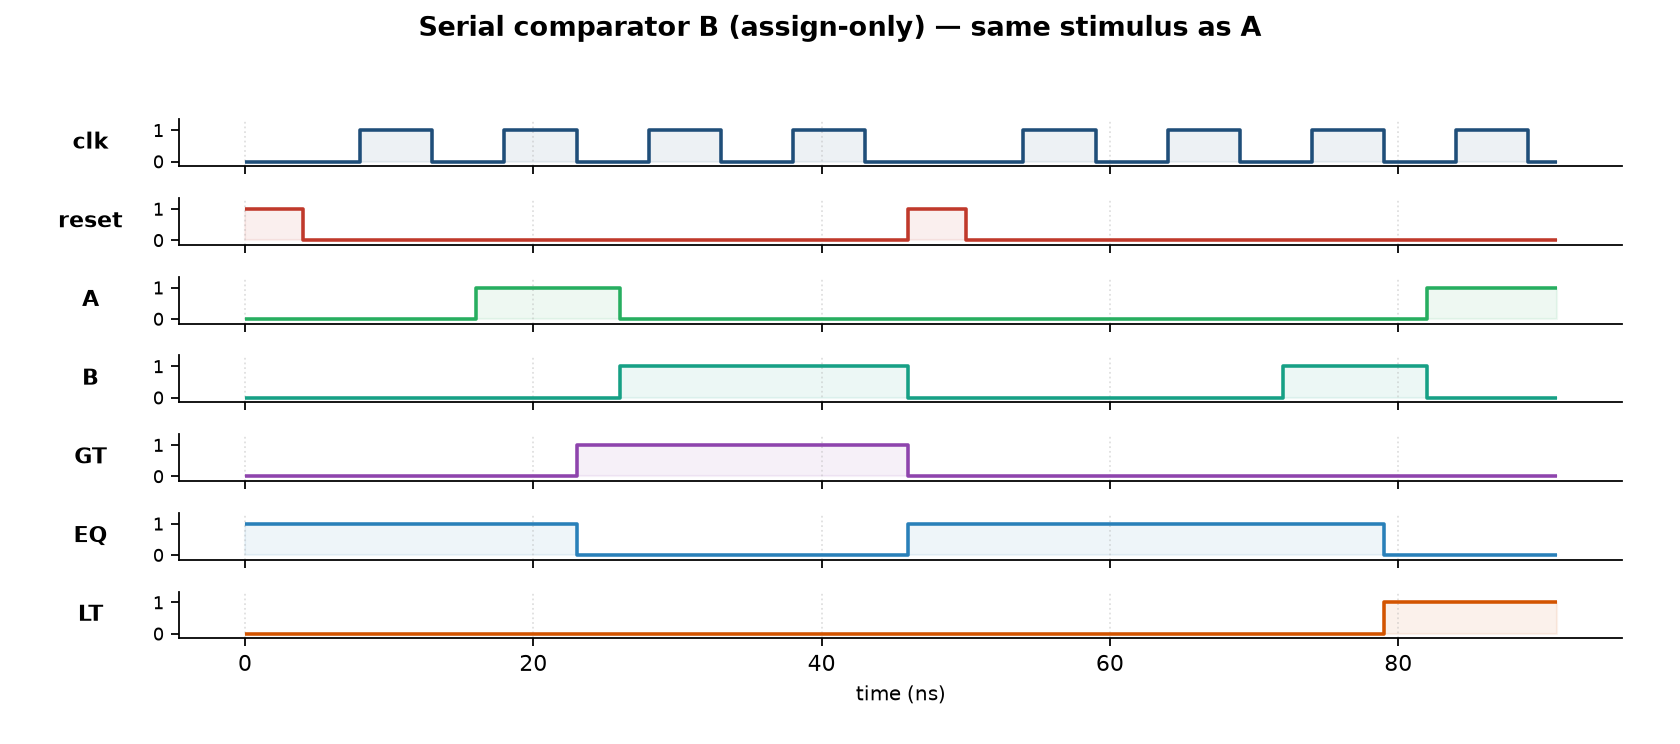
\includegraphics[width=\textwidth]{figs/wave_serial_assign.png}\\[0.4em]
{\small شکل ۲ --- نسخهٔ B (\lr{serial\_comparator\_assign}): فقط \lr{assign} (مسترـ‌اسلیو)}
\end{center}

\pagebreak
\subsubsection*{ردیابی دستی (برای ارائه)}

\textbf{مثال: مقایسه‌ی سریال $A{=}0100$ با $B{=}0011$} (MSB اول):

\begin{center}
\begin{tabular}{@{}cccccc@{}}
\toprule
\textbf{گام} & \textbf{A} & \textbf{B} & \textbf{پیشوند} & \textbf{نتیجه} & \textbf{GEL} \\
\midrule
reset & -- & -- & $\varepsilon$ & برابر & 010 \\
۱ & ۰ & ۰ & $0$ vs $0$ & برابر & 010 \\
۲ & ۱ & ۰ & $01$ vs $00$ & $A>B$ & 100 \\
۳ & ۰ & ۱ & (قفل) & $A>B$ & 100 \\
۴ & ۰ & ۱ & (قفل) & $A>B$ & 100 \\
\bottomrule
\end{tabular}
\end{center}

تصمیم در بیت ۲ گرفته می‌شود و تا آخر چسبنده می‌ماند -- دقیقا همان چیزی که سناریوی \lr{gt\_bit2} در تست‌بنچ بررسی می‌کند.

\subsubsection*{نتایج تست}

همه‌ی شبیه‌سازی‌ها با \lr{Icarus Verilog 12.0}:

\begin{center}
\begin{tabular}{@{}p{4.2cm}p{7.0cm}r@{}}
\toprule
\textbf{تست} & \textbf{پوشش} & \textbf{نتیجه} \\
\midrule
tb\_cascadable\_1bit & همه‌ی ۳۲ ترکیب ورودی ۵بیتی & 32/32 \\
tb\_comparator\_4bit & همه‌ی ۲۵۶ جفت $A,B\in\{0..15\}$ & 256/256 \\
tb\_serial (نسخه‌ی A) & نمونه‌ها + ریست وسط‌راه + exhaustive نهایی & 312/312 \\
tb\_serial (نسخه‌ی B) & همان بردارها روی ماژول فقط-\lr{assign} & 312/312 \\
\bottomrule
\end{tabular}
\end{center}

خروجی واقعی \lr{run\_tests.sh}:

\begin{latin}
\lstinputlisting[basicstyle=\ttfamily\scriptsize]{figs/test_run_output.txt}
\end{latin}

جمع کل: \textbf{۴ از ۴ مجموعه‌تست پاس، صفر شکست}.

\subsubsection*{نکات پیاده‌سازی}

\begin{itemize}
  \item در قسمت ۱ فقط \lr{assign} داخل بلوک ۱بیتی به کار رفته؛ ۴بیتی صرفا نمونه‌سازی ساختاری همان بلوک است (سلسله‌مراتبی مطابق خواسته‌ی آزمایش).
  \item در قسمت ۲ دو تفسیر از فقط جریان داده پیاده شد: A برای شبیه‌سازی/سنتز لبه‌حساس استاندارد، و B برای رعایت لفظی بدون توصیف دیگر با زوج \lr{latch} مسترـ‌اسلیو.
  \item ترتیب بیت‌ها \lr{MSB}-اول است؛ در غیر این صورت cascade/سریال با معنی عددی unsigned هم‌خوان نمی‌شود.
\end{itemize}

\end{document}
